%% This is file `elsarticle-template-1-num.tex',
%%
%% Copyright 2009 Elsevier Ltd
%%
%% This file is part of the 'Elsarticle Bundle'.
%% ---------------------------------------------
%%
%% It may be distributed under the conditions of the LaTeX Project Public
%% License, either version 1.2 of this license or (at your option) any
%% later version.  The latest version of this license is in
%%    http://www.latex-project.org/lppl.txt
%% and version 1.2 or later is part of all distributions of LaTeX
%% version 1999/12/01 or later.
%%
%% Template article for Elsevier's document class `elsarticle'
%% with numbered style bibliographic references
%%
%% $Id: elsarticle-template-1-num.tex 149 2009-10-08 05:01:15Z rishi $
%% $URL: http://lenova.river-valley.com/svn/elsbst/trunk/elsarticle-template-1-num.tex $
%%
\documentclass[preprint,12pt]{elsarticle}

%% Use the option review to obtain double line spacing
%% \documentclass[preprint,review,12pt]{elsarticle}

%% Use the options 1p,twocolumn; 3p; 3p,twocolumn; 5p; or 5p,twocolumn
%% for a journal layout:
%% \documentclass[final,1p,times]{elsarticle}
%% \documentclass[final,1p,times,twocolumn]{elsarticle}
%% \documentclass[final,3p,times]{elsarticle}
%% \documentclass[final,3p,times,twocolumn]{elsarticle}
%% \documentclass[final,5p,times]{elsarticle}
%% \documentclass[final,5p,times,twocolumn]{elsarticle}

%% The graphicx package provides the includegraphics command.
\usepackage{graphicx}
%% The amssymb package provides various useful mathematical symbols
\usepackage{amssymb}
\usepackage{amsmath}
%% The amsthm package provides extended theorem environments
%% \usepackage{amsthm}

%% The lineno packages adds line numbers. Start line numbering with
%% \begin{linenumbers}, end it with \end{linenumbers}. Or switch it on
%% for the whole article with \linenumbers after \end{frontmatter}.
\usepackage{lineno}

%% package for code quoting
\usepackage{listings}

%% natbib.sty is loaded by default. However, natbib options can be
%% provided with \biboptions{...} command. Following options are
%% valid:

%%   round  -  round parentheses are used (default)
%%   square -  square brackets are used   [option]
%%   curly  -  curly braces are used      {option}
%%   angle  -  angle brackets are used    <option>
%%   semicolon  -  multiple citations separated by semi-colon
%%   colon  - same as semicolon, an earlier confusion
%%   comma  -  separated by comma
%%   numbers-  selects numerical citations
%%   super  -  numerical citations as superscripts
%%   sort   -  sorts multiple citations according to order in ref. list
%%   sort&compress   -  like sort, but also compresses numerical citations
%%   compress - compresses without sorting
%%
%% \biboptions{comma,round}

% \biboptions{}

\journal{Udacity}

\begin{document}

\begin{frontmatter}

%% Title, authors and addresses

\title{Costa Rican Household Poverty Level Prediction with Deep Learning}

%% use the tnoteref command within \title for footnotes;
%% use the tnotetext command for the associated footnote;
%% use the fnref command within \author or \address for footnotes;
%% use the fntext command for the associated footnote;
%% use the corref command within \author for corresponding author footnotes;
%% use the cortext command for the associated footnote;
%% use the ead command for the email address,
%% and the form \ead[url] for the home page:
%%
%% \title{Title\tnoteref{label1}}
%% \tnotetext[label1]{}
%% \author{Name\corref{cor1}\fnref{label2}}
%% \ead{email address}
%% \ead[url]{home page}
%% \fntext[label2]{}
%% \cortext[cor1]{}
%% \address{Address\fnref{label3}}
%% \fntext[label3]{}


%% use optional labels to link authors explicitly to addresses:
%% \author[label1,label2]{<author name>}
%% \address[label1]{<address>}
%% \address[label2]{<address>}

\author{David Jansen}
%% \ead{dpmjansen@gmail.com}

\address{Groningen, Netherlands}

\begin{abstract}
%% Text of abstract
In this report, the performance of a Deep Neural Network (DNN) is compared against a Random Forest on the Costa Rican Household Poverty Level Prediction dataset using a macro F1 score. The DNN performs very poorly on the dataset compared to the Random Forest model. Issues regarding the performance of the model may have to do with the dataset. The dataset had a very low variance for over 110 of the 142 available features, which made it hard for the network to properly learn how to separate the data. Suggestions for improving the model include more extensive pre-processing of the data.
\end{abstract}

\begin{keyword}
Deep learning \sep 
\LaTeX \sep 
Prediction \sep 
Multi-class \sep 
Classification \sep
Kaggle
%% keywords here, in the form: keyword \sep keyword

\end{keyword}

\end{frontmatter}

%% main text
\section{Definition}
\label{S:1}

\subsection{Project Overview}

Accurately assessing social needs to ensure the poorest people our planet get the help they need is a difficult task. The Inter- American Development Bank (IADB) is an organization which focuses to improve the lives of those who live in Latin America and the Caribbean. Publications made in December 2016 by the IADB reveal that in 2015 between 8.2\% for Chili to 68.7\% of the total population of those countries live of less than 5 USD a day. Extreme cases of poverty range between 2.7\% for Chili and a shocking 32.6\% for Guatemala, where the income a day is less than 3.1 USD. In a study in 2015 a proposition was made to apply machine learning to poverty targeting (\citet{McBride:2015}). The study revealed that they were able to improve on the then standardized method for targeting applied by the USAID by 2 to 18 percent using a Random Forest algorithm. For this reason, the IADB is looking for new ways to reach people who are in need of help. They have reached out to the Kaggle community in order to find new ways to help identify vulnerable households who may need help.

\subsection{Problem Statement}

In Latin America, a Proxy Means Test (PMT) is used to asses the level of need a household needs. Despite this assessment being an improvement, a need for a model which more accurately classifies these households is present. The IADB has asked to Kaggle Community to create such a model. They have provided a dataset containing multiple characteristics of a Costa Rican household.

\subsection{Metrics}

For this project, a predefined metric was given. A macro F1 score will be used to determine the accuracy of the model. A F1 score is defined as a harmonic mean of precision and recall (\citet{Yutaka:2007}).\\

F1-score = $2\cdot\frac{Precision \cdot Recall}{Precision + Recall}$\\

This approach is not usable for a multi-class classification problem. The method chosen by the competition host is a variation of that called a macro-F1 score. It uses the F1 scores of all classes and divides it by the total number of possible classes as a resulting score.\\

macro F1 = $\frac{F1Class 1 + F1Class 2 + ... + F1 ClassN}{N}$\\

An important note added by the Competition host is that \textbf{only the heads of household are used in scoring}. All household members are included in test + the sample submission, but only heads of households are scored.

\section{Analysis}
\label{S:2}

\subsection{Data Exploration and Visualisation}
There are two files the IADB has provided. A training dataset containing multiple features including a target label feature and a test set containing the same features, but without the target label. The datasets respectively contain approximately nine thousand and twenty-four thousand data points. Due to the nature of the Kaggle competition, external data is not allowed.\\
The dataset contains the following core data fields (from Kaggle):
\begin{itemize}
\item Id - a unique identifier for each row.
\item Target - the target is an ordinal variable indicating groups of income levels.
\begin{itemize}
\item 1 = extreme poverty
\item 2 = moderate poverty
\item 3 = vulnerable households
\item 4 = non vulnerable households
\end{itemize}
\item idhogar - this is a unique identifier for each household. This can be used to create household-wide features, etc. All rows in
a given household will have a matching value for this identifier.
\item parentesco1 - indicates if this person is the head of the household.
\end{itemize}
The dataset contains a total of 143 columns.
An initial look at the data reveals that the data points are heavily skewed towards non-vulnerable households which are overrepresented in the data. Due to this class imbalance, care has to be taken when splitting the data for training and crossvalidation (Figure \ref{fig:class_imbalance_full}). This class imbalance is also present in the heads of household (Figure \ref{fig:class_imbalance}). Both oversampling and undersampling were experimented with in order to tackle this issue (See \ref{sss:balancing_dataset})

\begin{figure}[h!]
\centering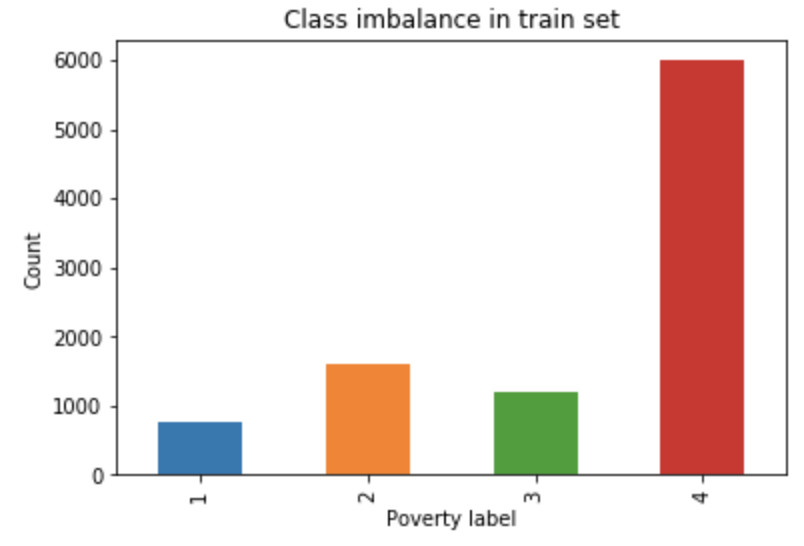
\includegraphics[width=0.8\linewidth]{class_imbalance_full}
\caption{Class imbalance in training data}
\label{fig:class_imbalance_full}
\end{figure}

\begin{figure}[h!]
\centering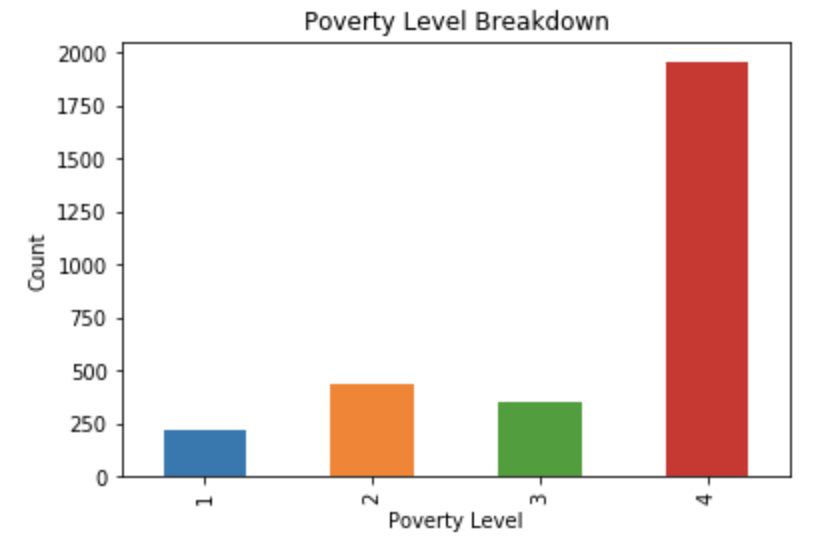
\includegraphics[width=0.8\linewidth]{class_imbalance}
\caption{Class imbalance for heads of household in training data}
\label{fig:class_imbalance}
\end{figure}

Another issue is invalid / missing data. This data needs to be cleaned up before it can presented to the prediction models (Figure \ref{fig:missing_datapoints}).

Furthermore, due to only the heads of household being considered relevant by the competition host, both the benchmarking Random Forest model and the DNN are trained using only data from heads of household. The dataset contains a feature which labels an individual as a head of household called 'parentesco1' which is used throughout the project to subset the data (after pre-processing).

%% \subsection{Exploration Visualization}
%% A visualization has been provided that summarizes or extracts a relevant characteristic or feature about the dataset or input data with thorough discussion. Visual cues are clearly defined.


\subsection{Algorithms and Techniques}

One could argue that using a macro F1 score is not the best choice for measuring. In python's sklearn package, a method for implementing the macro F1 score is available, however it states the following: "Calculate metrics for each label, and find their unweighted mean. \textbf{This does not take label imbalance into account}.". Due to the dataset having a label (or class) imbalance, this forces somehow getting rid of the class imbalance so the resulting measure can be more meaningful. The measure however is set by the competition host, and cannot be changed. 

\subsection{Benchmark}
For benchmarking, a Random Forest classifier was chosen to compete the neural network. In order to create a semi-competitive model, Grid Search was employed to select some of the hyper parameters. The resulting macro F1 score looked promising, although the model does show signs of overfitting (Table \ref{table:benchmark_F1}).

\begin{table}[]
\resizebox{\textwidth}{!}{
\begin{tabular}{ll}
\textbf{Dataset} & \textbf{macro F1 score}\\
Training          & 0.9299\\
Cross-validation     & 0.4153\\
Testing     & 0.3880\\
\end{tabular}
}
\caption{macro F1 score for benchmarking model}
\label{table:benchmark_F1}
\end{table}


\section{Methodology}
\label{S:3}

\subsection{Data Preprocessing}

Inspection of the testdata revealed four issues which needed to be addressed. Firstly, not all columns of the data were numerical fields, which is a requirement for both the benchmarking model and the deep neural network (\ref{sss:conversion}). Secondly, the data contained datapoints which were null. These datapoints needed to be corrected (\ref{sss:correct_null}). Thirdly, some columns revealed to have no variance in the data. These columns have been removed from the dataset (\ref{sss:removal}). Finally, there is class imbalance in the dataset. Label balancing is employed in order to reduce the presence of the overrepresented class (\ref{sss:balancing_dataset})

\subsection{Implementation}
\label{ss:implementation}
\subsubsection{Converting object to numerical}
\label{sss:conversion}
Inspection revealed that the datasets contained 5 columns which were non-numerical (Table \ref{table:non_numerical})\\

\begin{table}[]
\resizebox{\textwidth}{!}{
\begin{tabular}{ll}
\hline
column name & description                                                                                                                                             \\ \hline
Id          & rowId                                                                                                                                                   \\
idhogar     & Household level identifier                                                                                                                              \\
dependency  & fraction of household members who are dependent on non-dependent                  \\
edjefe      & years of education of male head of household\\
edjefa      & years of education of female head of household\\ \hline
\end{tabular}
}
\caption{Object types in the dataset}
\label{table:non_numerical}
\end{table}

Both the 'Id' and the 'idhogar' column were not converted, due to the values not being useful for this particular prediction problem. In the description of both 'edjefe' and 'edjefa' could be found that yes and no should be 1 and - respectively. These two columns have been remapped and converted to int32. The 'dependency' column contained the same type of data ('yes' and 'no') and was remapped aswell. This column however contained floating point integers and was therefor not converted to int32 but float64 instead.

\subsubsection{Correcting null values}
\label{sss:correct_null}
A method in python is used to inspect a given dataframe to reveal any missing (null) values (Listing \ref{code:missing_data})

\begin{lstlisting}[language=Python, label={code:missing_data}, caption={Analyze dataset for missing values}]
def get_missing(df):
    """
    Analyze missing values in dataframe:
    """
    # Number of missing in each column
    missing = pd.DataFrame(df.isnull().sum()).rename(columns = {0: 'total'})
    # Create a percentage missing
    missing['percent'] = missing['total'] / len(df)
    # Drop columns where everything is present
    missing = missing[missing.total != 0]
    return missing
\end{lstlisting}

In Figure \ref{fig:missing_datapoints} the missing datapoints can be seen.

For each of the feature, different measures were taken to clean the data. rez{\_}esc which represents the years behind in school was only collected for individuals who's age ranged between 7 and 19 years. The missing datapoints seemed to mostly exist out of this age range and were corrected to 0. Missing data was also present for individuals of age 18 (and a single one of age 10). The individuals of age 18 were corrected by getting the mean rez{\_}esc for the nearest age group (age 17). The individual of age 10 was corrected by using the mean of the same age group. v18q1 which represents the number of tablets a household owns was corrected by setting all the values to 0. This is done because another feature called v18q which represents whether a household has a tablet or not, revealed that for every v18q = 0, v18q1 was missing. v2a1, which represents the monthly rent payment, was corrected in two stages. Firstly, there are accompanying features which have to do with the type of household payment there is. The first correction taken place was to set v2a1 to 0 for every household which fully owns its house. Secondly, the other missing datapoints were all grouped by two other household payment type markers (tipovivi4 and tipovivi5). Due to both of these markers not having any rent data associated with it, it was unknown what the actual value the coresponding v2a1 should have. This is also confirmed by the competition host on the discussion board. Due to this, the v2a1 was set to 0 for both these household payment type markers. Finally the 5 missing datapoints for meaneduc (and its squared accompanying feature SQBmeaned), which represents the average years of education for adults in the houshold was corrected by setting it to the average years of education of the individual. This value was squared for SQBmeaned.

\begin{figure}[h]
\centering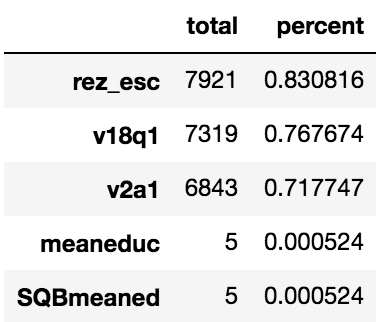
\includegraphics[width=0.4\linewidth]{missing_values}
\caption{Missing datapoints}
\label{fig:missing_datapoints}
\end{figure}

\subsubsection{Removal of columns correction}
\label{sss:removal}

The python \textit{sklearn} library comes with a class which can help removing features with low or no variance. The implementation of the class set the variance threshold to 1.0, dropping features which have a lower variance.

\begin{lstlisting}[language=python,label={code:feature_removal},caption={Using VarianceThreshold to remove features}]
from sklearn.feature_selection import VarianceThreshold

sel = VarianceThreshold(threshold=1.0)
sel = sel.fit(X)
remaining_columns_ix = sel.get_support(indices=True)
X_train_transformed = sel.transform(X)
test_transformed = sel.transform(test_drp)
\end{lstlisting}

Utilizing this class the dataset was downsized to only 28 columns. It decreased the amount of overfitting done by the Random Forest benchmark model by 2\%

\subsubsection{Balancing of the dataset}
\label{sss:balancing_dataset}

Initial analysis of the data revealed that the data was heavily skewed due to one of the classes being overrepresented in the data. The training dataset reconfirms this finding (Figure \ref{fig:class_imbalance}).

Utilizing another python library called \textit{imblearn}, the data was transformed into a balanced set (Listing \ref{code:balancing};Figure \ref{fig:balanced_dataset}).

\begin{lstlisting}[language=Python,label={code:balancing},caption={Balance dataset in python}]
from imblearn.over_sampling import RandomUnderSampler

smp = RandomUnderrSampler(random_state=42)
X_res, y_res = smp.fit_sample(X, y)
\end{lstlisting}

\begin{figure}[!h]
\centering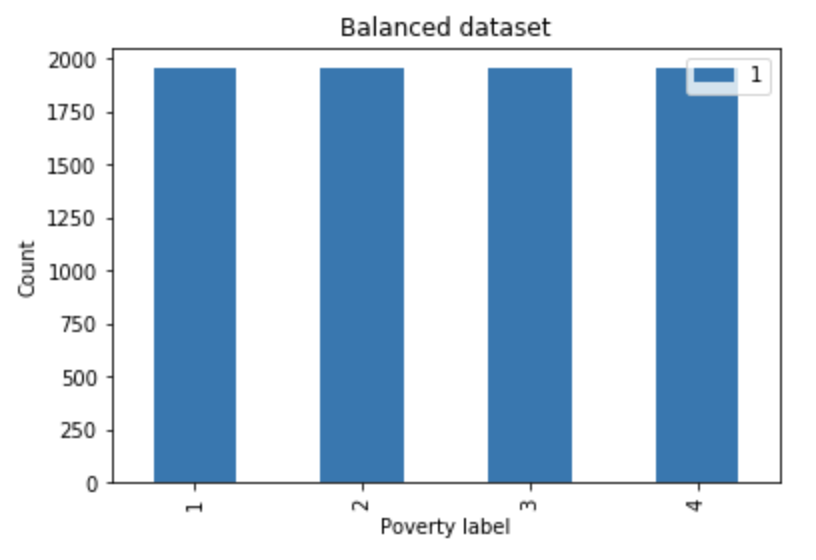
\includegraphics[width=0.8\linewidth]{balanced_dataset}
\caption{Training data after balancing}
\label{fig:balanced_dataset}
\end{figure}

\subsection{Refinement}
As stated, a deep neural network was created in order to compete the benchmarking model. The earliest model consisted of a total of four layers, an input layer, two hidden layers and an output layer (Listing \ref{code:dnn1}).

\begin{lstlisting}[language=Python, label={code:dnn1},caption={Earliest Deep Neural Network}]
model = Sequential()

model.add(Dense(64, input_dim=X_train.shape[1], activation='relu'))
model.add(Dropout(0.20))
model.add(Dense(32 ,activation='relu'))
model.add(Dropout(0.20))
model.add(Dense(32 ,activation='relu'))
model.add(Dropout(0.20))
model.add(Dense(y_train_encoded.shape[1], activation='relu')) # back to one-hot-encoded result

model.summary()
\end{lstlisting}

The model was created using ways to reduce overfitting a bit by adding dropout layers\cite{Srivastava:2014} and using a ReLU activation function. 

The first finding was, that this somehow caused unusual output. Specifically, the outputs were all zero's. A Stanford Course on using Convolutional Neural Networks for Visual Recognition reveals that "Unfortunately, ReLU units can be fragile during training and can "die". For example, a large gradient flowing through a ReLU neuron could cause the weights to update in such a way that the neuron will never activate on any datapoint again. If this happens, then the gradient flowing through the unit will forever be zero from that point on."\cite{CSN:ReLU}. Changing the activation function from ReLU to tanh solved this issue. An alternative method would be to use LeakyReLU activators.
A second improvement was made by adding batch normalization. Batch Normalization should improve the training speed (\citet{Ioffe:2015}), however the model also slightly improved in its macro F1 score by applying it. Increasing the amount of 'units' in each layer also proved to increase the performance up to a certain amount. Increasing the amount of Dense layers in the network seems to somewhat stabilize the final result, however it did not improve the resulting score.

Some variations of the model increased the amount of neurons and layers. Increasing the amount of neurons improved the performance. Adding additional layers additionally improved the performance, but only up to a certain point before it started having diminishing returns.

The final model can be seen in Listing \ref{code:dnn_final}

\begin{lstlisting}[language=Python, label={code:dnn_final},caption={Final Deep Neural Network}]
model = Sequential()

model.add(Dense(256, input_dim=X_train.shape[1], activation='tanh'))
model.add(Dropout(0.2))
model.add(BatchNormalization())
model.add(Dense(512 ,activation='tanh'))
model.add(Dropout(0.2))
model.add(BatchNormalization())
model.add(Dense(256 ,activation='tanh'))
model.add(Dropout(0.2))
model.add(BatchNormalization())
model.add(Dense(128 ,activation='tanh'))
model.add(Dropout(0.2))
model.add(BatchNormalization())
model.add(Dense(64 ,activation='tanh'))
model.add(Dropout(0.2))
model.add(BatchNormalization())
model.add(Dense(y_train_encoded.shape[1], activation='relu')) # back to one-hot-encoded result

model.summary()
\end{lstlisting}

\section{Results}
\label{S:4}

\subsection{Model Evaluation and Validation}

The final model consists of 6 Dense layers, 5 Dropout layers and 5 BatchNormalization layers. the activation layers were changed from ReLU to tanh to prevent the 'dead' ReLU problem, where all of the results ended up as 0. The final activation layer was kept as ReLU, to reduce the amount of label misses. Tanh activation allows values to get negative, which cannot be used in the prediction. The result of the model would vary between runs. With a standard deviation of 3\% and an almost 20\% variation between worst and best run the model cannot be considered stable. It does however have a mean which seems consistent over most of the runs (Figure \ref{fig:dnn_f1_comparison} and Figure \ref{fig:dnn_f1_comparison_plot}).

\begin{figure}[!h]
\centering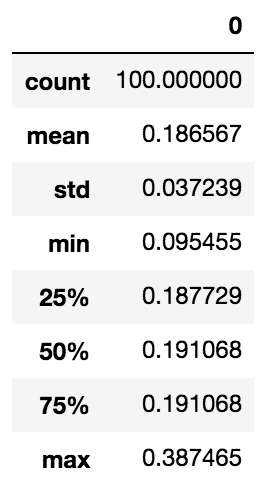
\includegraphics[width=0.3\linewidth]{dnn_f1_comparison}
\caption{Statistics for the neural network}
\label{fig:dnn_f1_comparison}
\end{figure}

\begin{figure}[!h]
\centering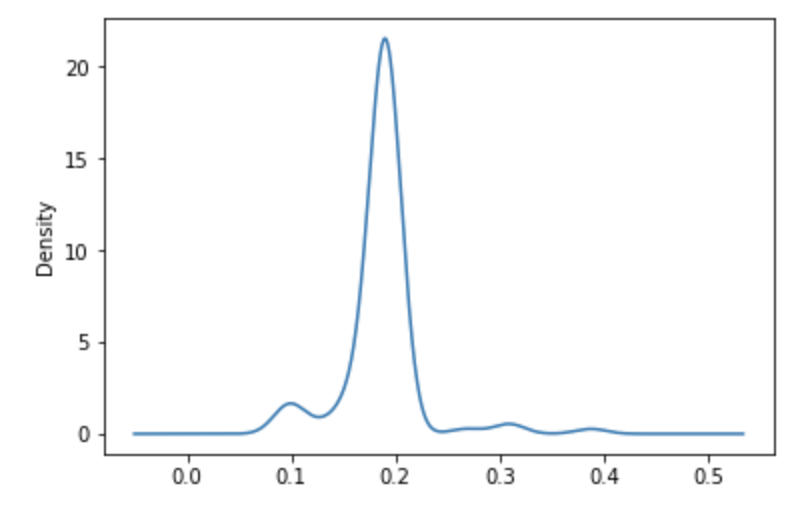
\includegraphics[width=0.8\linewidth]{dnn_f1_comparison_plot}
\caption{Statistics plot}
\label{fig:dnn_f1_comparison_plot}
\end{figure}

\subsection{Justification}

\begin{table}[]
\begin{tabular}{lll}
\textbf{Dataset} & \textbf{macro F1 Random Forest} & \textbf{macro F1 DNN}\\
Training & 0.9299 & 0.00 \\
Cross-validation & 0.4153 & 0.00 \\
Testing & 0.3880 & 0.00
\end{tabular}
\caption{macro F1 score comparison}
\label{table:comparison_F1}
\end{table}
The final results are compared to the benchmark result or threshold with some type of statistical analysis. Justification is made as to whether the final model and solution is significant enough to have adequately solved the problem.

\section{Conclusion}
\label{S:5}

\subsection{Free-Form Visualization}
A visualization has been provided that emphasizes an important quality about the project with thorough discussion. Visual cues are clearly defined.

\subsection{Reflection}
Using a deep neural network for predicting this problem did not proof to be a good solution. Partially this may be because of the data, and quite possibly also the model. I still struggle with is coming up with a design for a neural network. Although there is a lot of information online about neural networks, most of it is used for computer vision. It seems there are no concrete steps in building one, and that advice is mostly given in heuristics like ''don't overcomplicate it'. I did learn a couple of interesting things about the design. One thing that surprised me was the 'dead' ReLU problem where predictions were all 0, which did not conform for any situation. Some online material on this was helpful. Another surprise was the effect either oversampling or undersampling had on the resulting macro F1 score. In general, there is a lot for me to still learn in this area, both in Data Science and Machine Learning. I am positive I will keep on improving my skills for the future.

\subsection{Improvement}
The biggest problem I found was that it was hard for the model to separate the data. One improvement would be to spent more time in pre-processing the data, this would take some time however. Additionally, not using a neural network but a more conventional machine learning algorithm might prove to be a better idea. An additional improvement would be to stabilize the model more. While running simulations, the resulting macro F1 score could differ by approximately 0.10 between runs, without the model changing.

%% The Appendices part is started with the command \appendix;
%% appendix sections are then done as normal sections
%% \appendix

%% \section{}
%% \label{}

%% References
%%
%% Following citation commands can be used in the body text:
%% Usage of \cite is as follows:
%%   \cite{key}          ==>>  [#]
%%   \cite[chap. 2]{key} ==>>  [#, chap. 2]
%%   \citet{key}         ==>>  Author [#]

%% References with bibTeX database:
\appendix
\bibliographystyle{model1-num-names}
\bibliography{capstone-bibtex.bib}

%% Authors are advised to submit their bibtex database files. They are
%% requested to list a bibtex style file in the manuscript if they do
%% not want to use model1-num-names.bst.

%% References without bibTeX database:

% \begin{thebibliography}{00}

%% \bibitem must have the following form:
%%   \bibitem{key}...
%%

% \bibitem{}

% \end{thebibliography}

\end{document}

%%
%% End of file `elsarticle-template-1-num.tex'.

%% 0.1480 f1 macro of benchmark with undersampled dataset
%% 0.1788 f1 macro of benchmark with oversampled dataset
